%-----------------------------------LICENSE------------------------------------%
%   This file is part of tikz_figures.                                         %
%                                                                              %
%   tikz_figures is free software: you can redistribute it and/or              %
%   modify it it under the terms of the GNU General Public License as          %
%   published by the Free Software Foundation, either version 3 of the         %
%   License, or (at your option) any later version.                            %
%                                                                              %
%   tikz_figures is distributed in the hope that it will be useful,            %
%   but WITHOUT ANY WARRANTY; without even the implied warranty of             %
%   MERCHANTABILITY or FITNESS FOR A PARTICULAR PURPOSE.  See the              %
%   GNU General Public License for more details.                               %
%                                                                              %
%   You should have received a copy of the GNU General Public License along    %
%   with tikz_figures.  If not, see <https://www.gnu.org/licenses/>.           %
%------------------------------------------------------------------------------%

% Use the standalone class for displaying the tikz image on a small PDF.
\documentclass[crop, tikz]{standalone}

% Import the tikz package to use for the drawing.
\usepackage{tikz}

% The arrows package is used for the LaTeX arrow.
\usetikzlibrary{arrows.meta}

% Begin the document.
\begin{document}

    % Begin the drawing.
    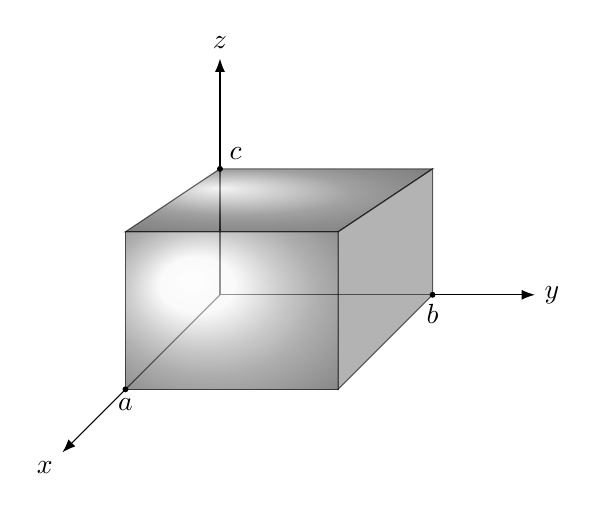
\begin{tikzpicture}[%
        line width = 0.4pt,
        line cap = round,
        > = Latex
    ]

        % Label the coordinate axes.
        \draw[->] (0, 0) to ( 4, 0) node[right] {$y$};
        \draw[->] (0, 0) to ( 0, 3) node[above] {$z$};
        \draw[->] (0, 0) to (-2,-2) node[below left] {$x$};

        % Three faces for the rectangular prism.
        \draw[ball color = gray!10!white, opacity = 0.6]
            (-1.2, -1.2) to (1.5, -1.2) to (1.5, 0.8) to (-1.2, 0.8) to cycle;
        \draw[ball color = gray!90!white, opacity = 0.6]
            (-1.2, 0.8) to (0.0, 1.6) to (2.7, 1.6) to (1.5, 0.8) to cycle;
        \draw[fill = gray, opacity = 0.6]
            (1.5, 0.8) to (2.7, 1.6) to (2.7, 0.0) to (1.5, -1.2) to cycle;

        % Nodes for the three points, three of the vertices of the prism.
        \draw[fill = black] (-1.2, -1.2) circle (0.03) node [below] {$a$};
        \draw[fill = black] (0.0, 1.6) circle (0.03) node [above right] {$c$};
        \draw[fill = black] (2.7,0) circle (0.03) node [below] {$b$};
    \end{tikzpicture}
\end{document}
